\documentclass{beamer}
%\usepackage{beamerthemeAmsterdam}
\usepackage{amsmath}
\usepackage{graphicx}

\title{JPEG-2000}
\subtitle{De Wondere Wereld van Wavelets}
\author{Jan Westerdiep \and Okke van Garderen}
\date{\today}
\institute{Universiteit van Amsterdam}

\begin{document}

\frame{\titlepage}

\section{Intro}
\frame{
  \frametitle{Vakantieplaatje}
  \begin{columns}
    \begin{column}{0.5\textwidth}
      \hfill
      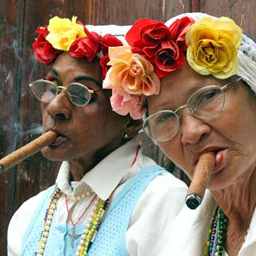
\includegraphics[width=\textwidth]{cigar.png}
      \hfill
    \end{column}
\pause
    \begin{column}{0.5\textwidth}
      \hfill
      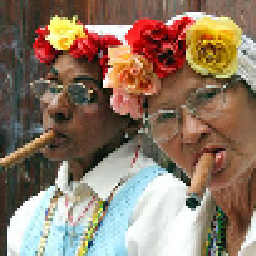
\includegraphics[width=\textwidth]{cigar_downscale.png}
      \hfill
    \end{column}
  \end{columns}
}
\frame{
  \frametitle{Vakantieplaatje}
  \begin{columns}
    \begin{column}{0.5\textwidth}
      \hfill
      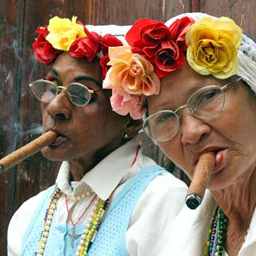
\includegraphics[width=\textwidth]{cigar.png}
      \hfill
    \end{column}
    \begin{column}{0.5\textwidth}
      \hfill
      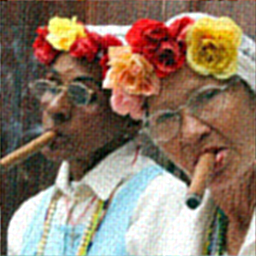
\includegraphics[width=\textwidth]{cigar_fourier.png}
      \hfill
    \end{column}
  \end{columns}
}
\frame{
  \frametitle{Vakantieplaatje}
  \begin{columns}
    \begin{column}{0.5\textwidth}
      \hfill
      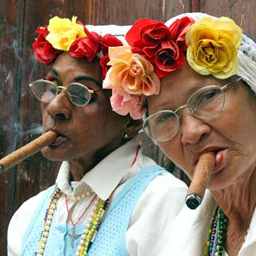
\includegraphics[width=\textwidth]{cigar.png}
      \hfill
    \end{column}
    \begin{column}{0.5\textwidth}
      \hfill
      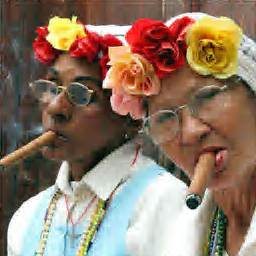
\includegraphics[width=\textwidth]{cigar_db2.png}
      \hfill
    \end{column}
  \end{columns}
}

\frame{
	\frametitle{Ons project}
	\begin{itemize}
		\item Beeldcompressie
		\item JPEG: Fouriertransformatie
		\item JPEG-2000: Wavelettransformatie
	\end{itemize}
}

\frame{
	\frametitle{Fouriertransformatie}
	\begin{itemize}
		\item Beginsignaal $f$
		\item Transformatie is omschrijven naar andere basis (sinussen en cosinussen)
		\begin{itemize}
			\item Voorbeeld: $\pi$ schrijven in termen van machten van tien (decimale ontwikkeling)
		\end{itemize}
		\item GIFje Fouriertransform.gif?
		\item Compressie door minst significante termen weg te laten
		\begin{itemize}
			\item $\pi \simeq 3.1415$ is `wel precies genoeg'
		\end{itemize}
		\item Nadeel: werkt niet goed bij plaatjes met scherpe randen
	\end{itemize}
}

\frame{
	\frametitle{Wavelettransformatie}
	\begin{itemize}
		\item Weer omschrijven in een andere basis
		\item Heel veel soorten wavelets
		\item (Wiskundig wat interessanter: relatief nieuw)
	\end{itemize}
}

\frame{
	\frametitle{Plaatjens}
}

\frame{
	\frametitle{Filmpjens}
}
\end{document}
